\section{Simulating The Great Recession}


\subsection{Model vs Data}

%This section demonstrates that unemployment scarring can reconcile the sluggish recovery from The Great Recession. 
In this section, I quantify the extent to which unemployment scarring explains the sluggish recovery from the Great Recession. In particular, I demonstrate that unemployment scarring explains a large share of the sluggish recovery from the Great Recession. To illustrate this, I simulate consumption and output during and after The Great Recession by estimating a sequence of negative demand shocks that allows the model to match the path of unemployment from 2008 to 2018. I perform this exercise in both the baseline HANK model with scarring and the HANK model without scarring. I then compare the untargeted paths of consumption and output to their empirical counterparts. I use data on consumption (real PCE), output (Real GDP), prices (PCE deflator), nominal wages (average earnings of private production employees), real hourly and real aggregate labor compensation (labor compensation from wages and salaries). I de-trend each series from the first quarter of 1990 to the last quarter of 2019 and then scale them down such that they represent deviations from the first quarter of 2008. 


\begin{figure}[H]
\begin{center}
\begin{minipage}{0.5\textwidth}
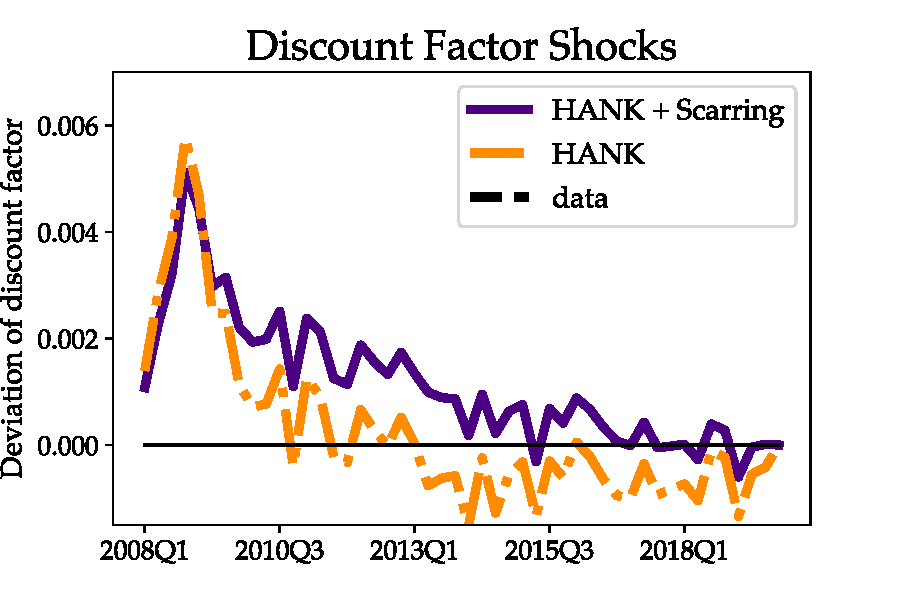
\includegraphics[scale=.5]{text/chapter1/Figures/GR_sim/DiscFacShks}
\end{minipage}\hspace*{\fill}
\begin{minipage}{0.5\textwidth}
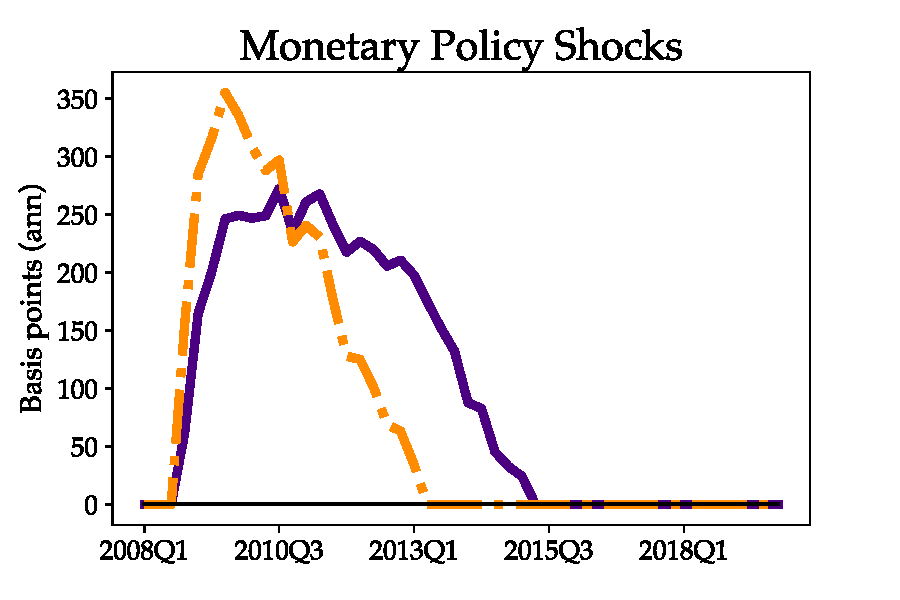
\includegraphics[scale=.5]{text/chapter1/Figures/GR_sim/EVShocks}
\end{minipage}
\medskip
\begin{minipage}{0.5\textwidth}
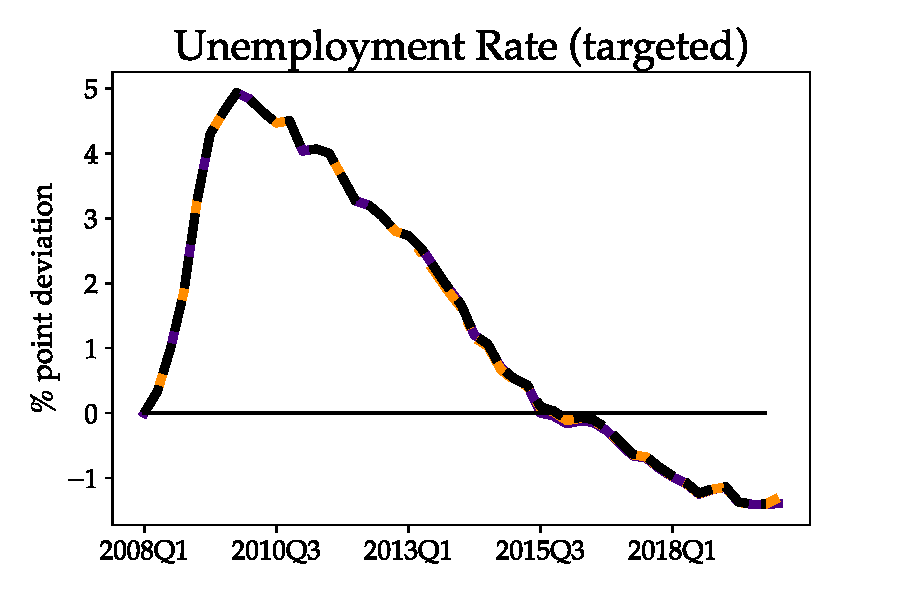
\includegraphics[scale=.5]{text/chapter1/Figures/GR_sim/Urate_}
\end{minipage}\hspace*{\fill}
\begin{minipage}{0.5\textwidth}
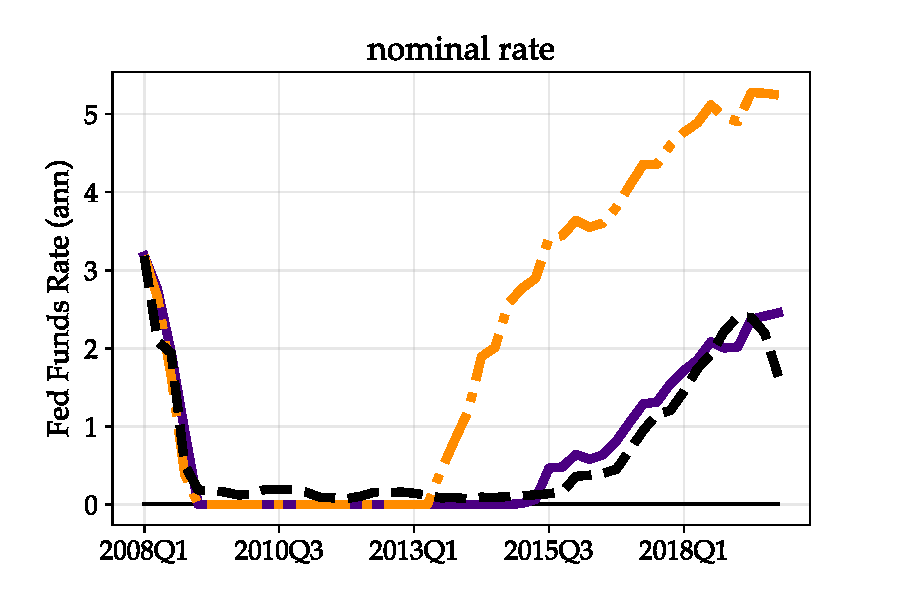
\includegraphics[scale=.5]{text/chapter1/Figures/GR_sim/FedFunds}
\end{minipage}
\caption{Estimated shocks to discount factor and nominal rate} 
\label{Estimatedshks}
\end{center}
\end{figure}


For the estimation, I follow \cite{kekre2023} and jointly estimate a sequence of discount factor shocks to match the path of unemployment from 2008 to 2018 monetary policy shocks to account for the zero lower bound. I use discount factor shocks for parsimony as the goal of this exercise is not to answer what caused The Great Recession but to answer why did The Great Recession lead to such a slow recovery\footnote{The same simulation exercise can be reproduced with shocks to the household borrowing limit or to the job separation rate and would not affect the results below as unemployment scarring is present in the responses to all aggregate shocks in the model.}. For these discount factor shocks, I set the fiscal adjustment parameter to $\phi_{b} = 0.015$, the lower bound of the estimates documented by  \cite{AuclertMicroJumpsMacroHumps}, and assume that the government cannot adjust taxes for 40 quarters to obtain a more accurate assessment of the effects of the Great Recession on debt. When estimating these discount factor shocks, I assume all discount factors follow an AR(1) with quarterly persistence 0.95. As noted in \cite{kekre2023}, the chosen AR(1) persistence does not alter the results as a different persistence will alter the estimated sequences of shocks but not the path of unemployment as that is what is targeted. The monetary policy shocks are assumed to have no persistence. I repeat this procedure over a grid of different wage rigidities $\phi_{w}$ and choose the wage rigidity parameter that minimizes the squared distance between the response of price index and its counterpart in the data. To capture the effects of unemployment scarring, I repeat this procedure for the version of the model where unemployment scarring is turned off in the same manner as in section 6. 


\begin{figure}[H] % "[t!]" placement specifier just for this example
\centering
\begin{minipage}{0.51\textwidth}
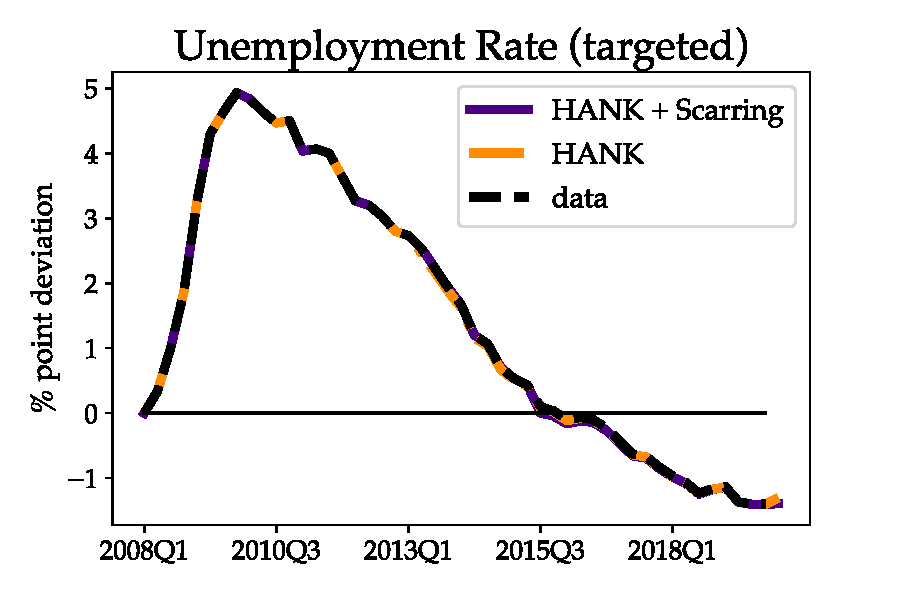
\includegraphics[scale=.55]{text/chapter1/Figures/GR_sim/Urate}
 \label{fig:a}
\end{minipage}\hspace*{\fill}
\begin{minipage}{0.51\textwidth}
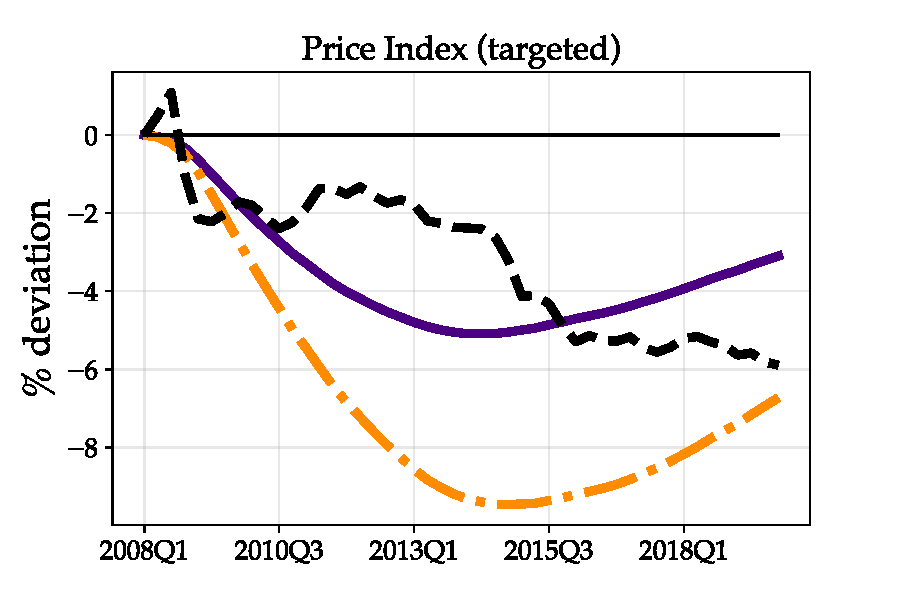
\includegraphics[scale=.55]{text/chapter1/Figures/GR_sim/PCE_defl}
 \label{fig:b}
\end{minipage}

\medskip
\begin{minipage}{0.51\textwidth}
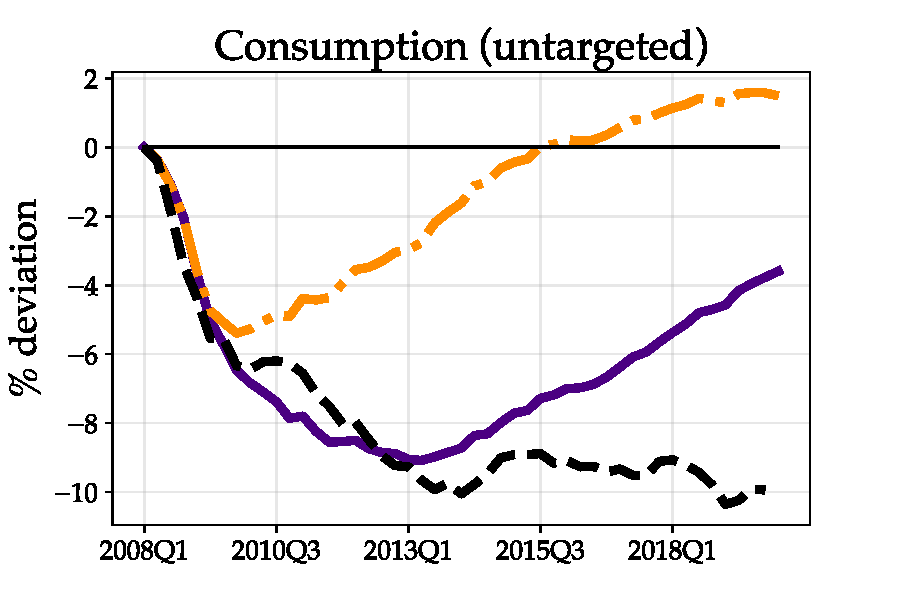
\includegraphics[scale=.55]{text/chapter1/Figures/GR_sim/PCE_IPR}
\label{fig:c}
\end{minipage}\hspace*{\fill}
\begin{minipage}{0.51\textwidth}
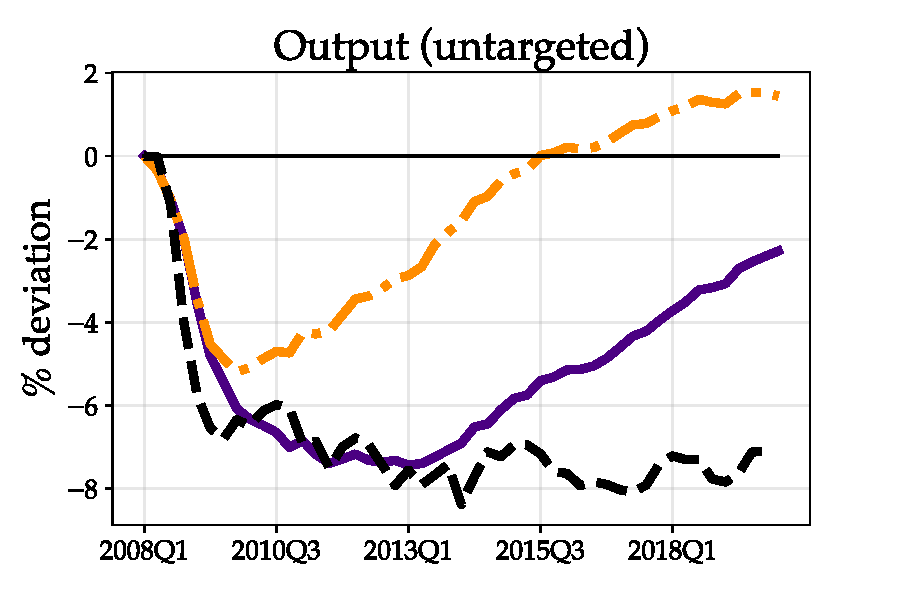
\includegraphics[scale=.55]{text/chapter1/Figures/GR_sim/GDP}
 \label{fig:d}
\end{minipage}

\medskip
\begin{minipage}{0.51\textwidth}
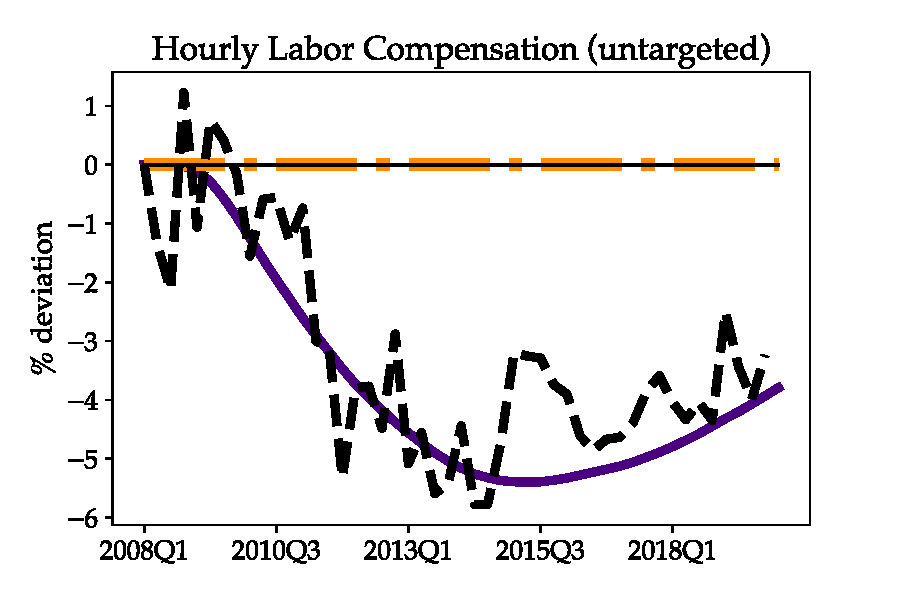
\includegraphics[scale=.55]{text/chapter1/Figures/GR_sim/Real_hourly_comp}
 \label{fig:e}
\end{minipage}\hspace*{\fill}
\begin{minipage}{0.51\textwidth}
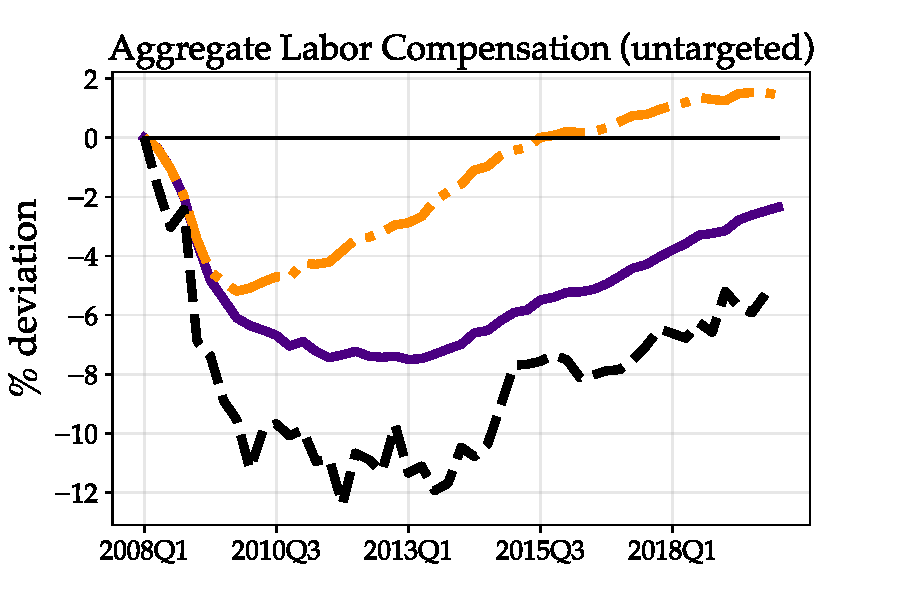
\includegraphics[scale=.55]{text/chapter1/Figures/GR_sim/labor_compensation}
 \label{fig:f}
\end{minipage}
\caption{Great Recession: Model vs Data (detrended)}
\floatfoot{Note: This figure compares the paths of various aggregates in the model with and without unemployment scarring to the data. The series display deviation from steady state for the model and from 2008Q1 for the data. In the data, real PCE, PCE deflator, real GDP, real hourly labor compensation, aggregate labor compensation are detrended from 1990Q1 to 2019Q4 and then rescaled such that the data represent deviation from 2008Q1.}
\label{NonTarget}
\end{figure}



\begin{figure}[H] % "[t!]" placement specifier just for this example
\centering
\begin{minipage}{0.51\textwidth}
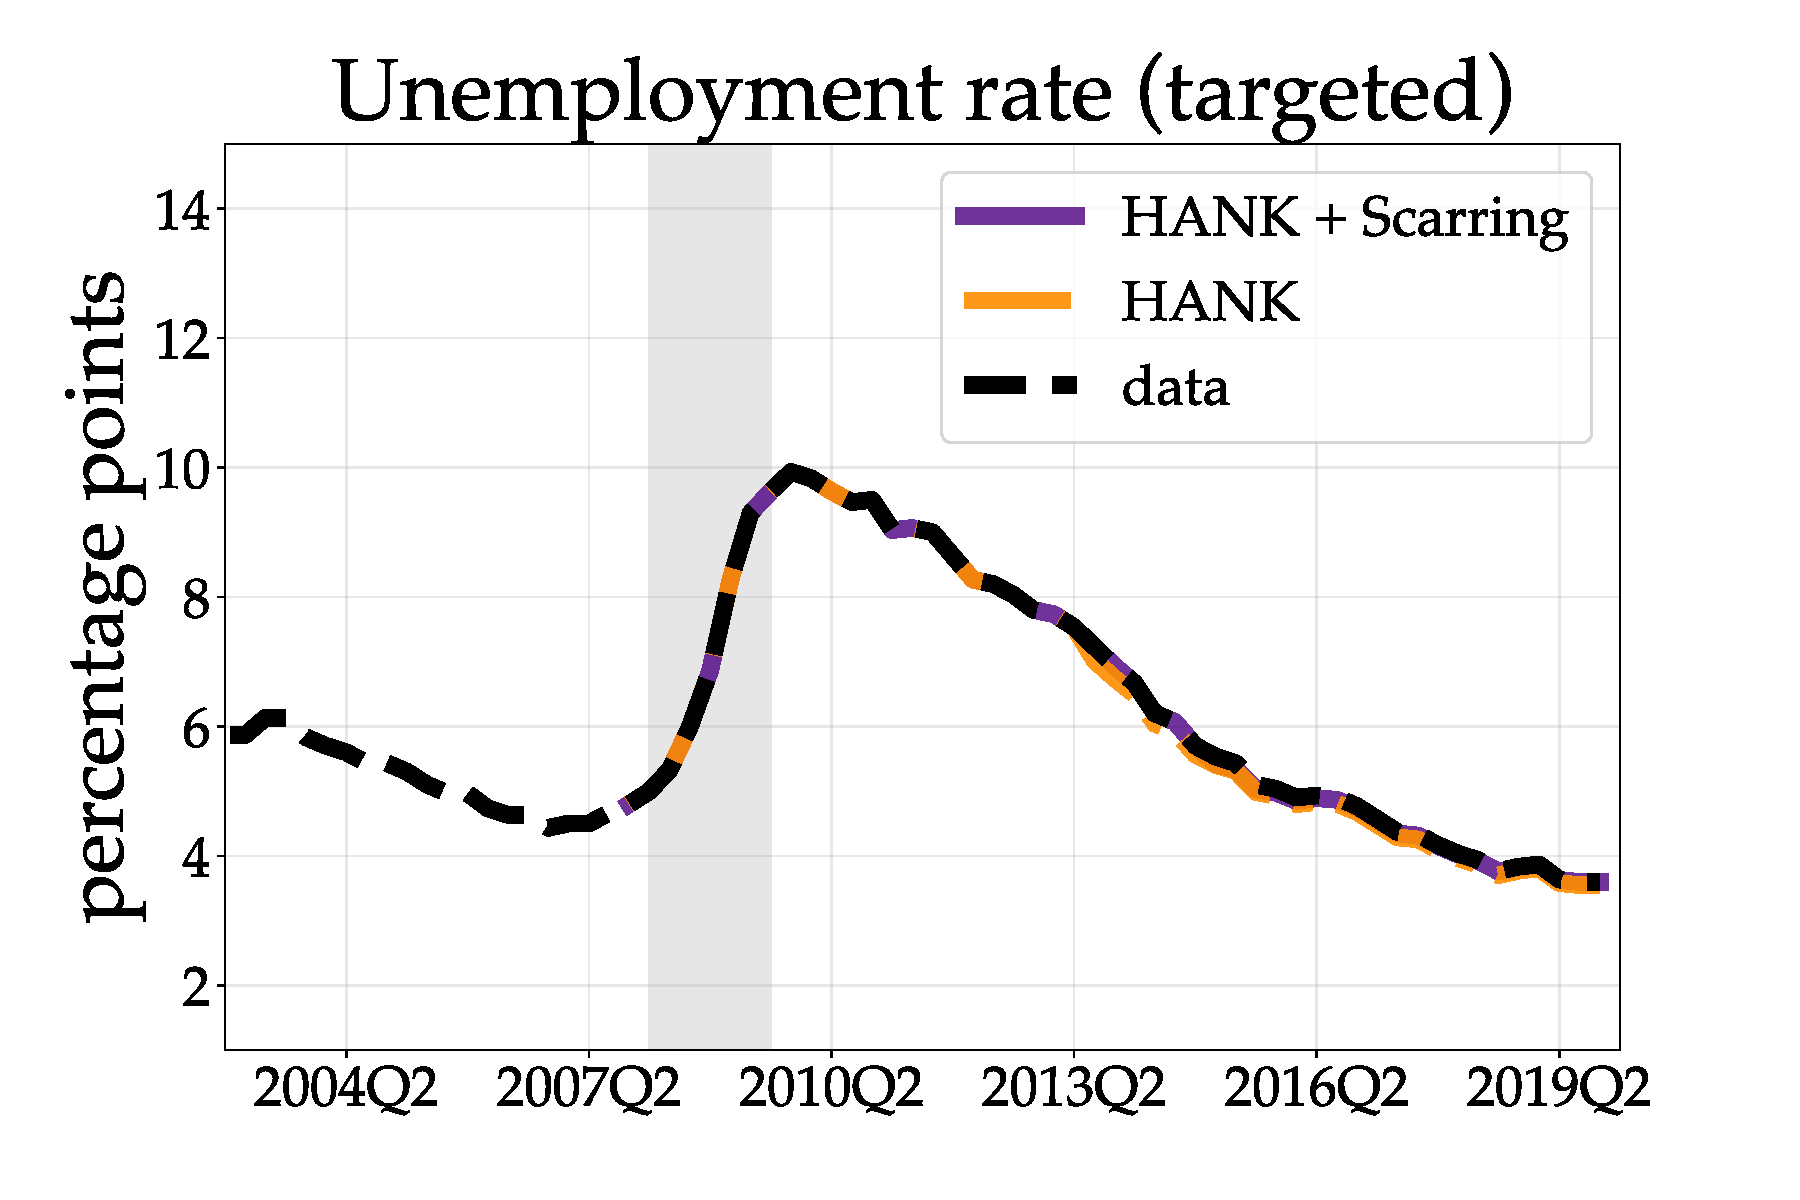
\includegraphics[scale=.29]{text/chapter1/Figures/GR_sim/Cleaner/Urate_vs_data_large_new}
 \label{fig:a}
\end{minipage}\hspace*{\fill}
\begin{minipage}{0.51\textwidth}
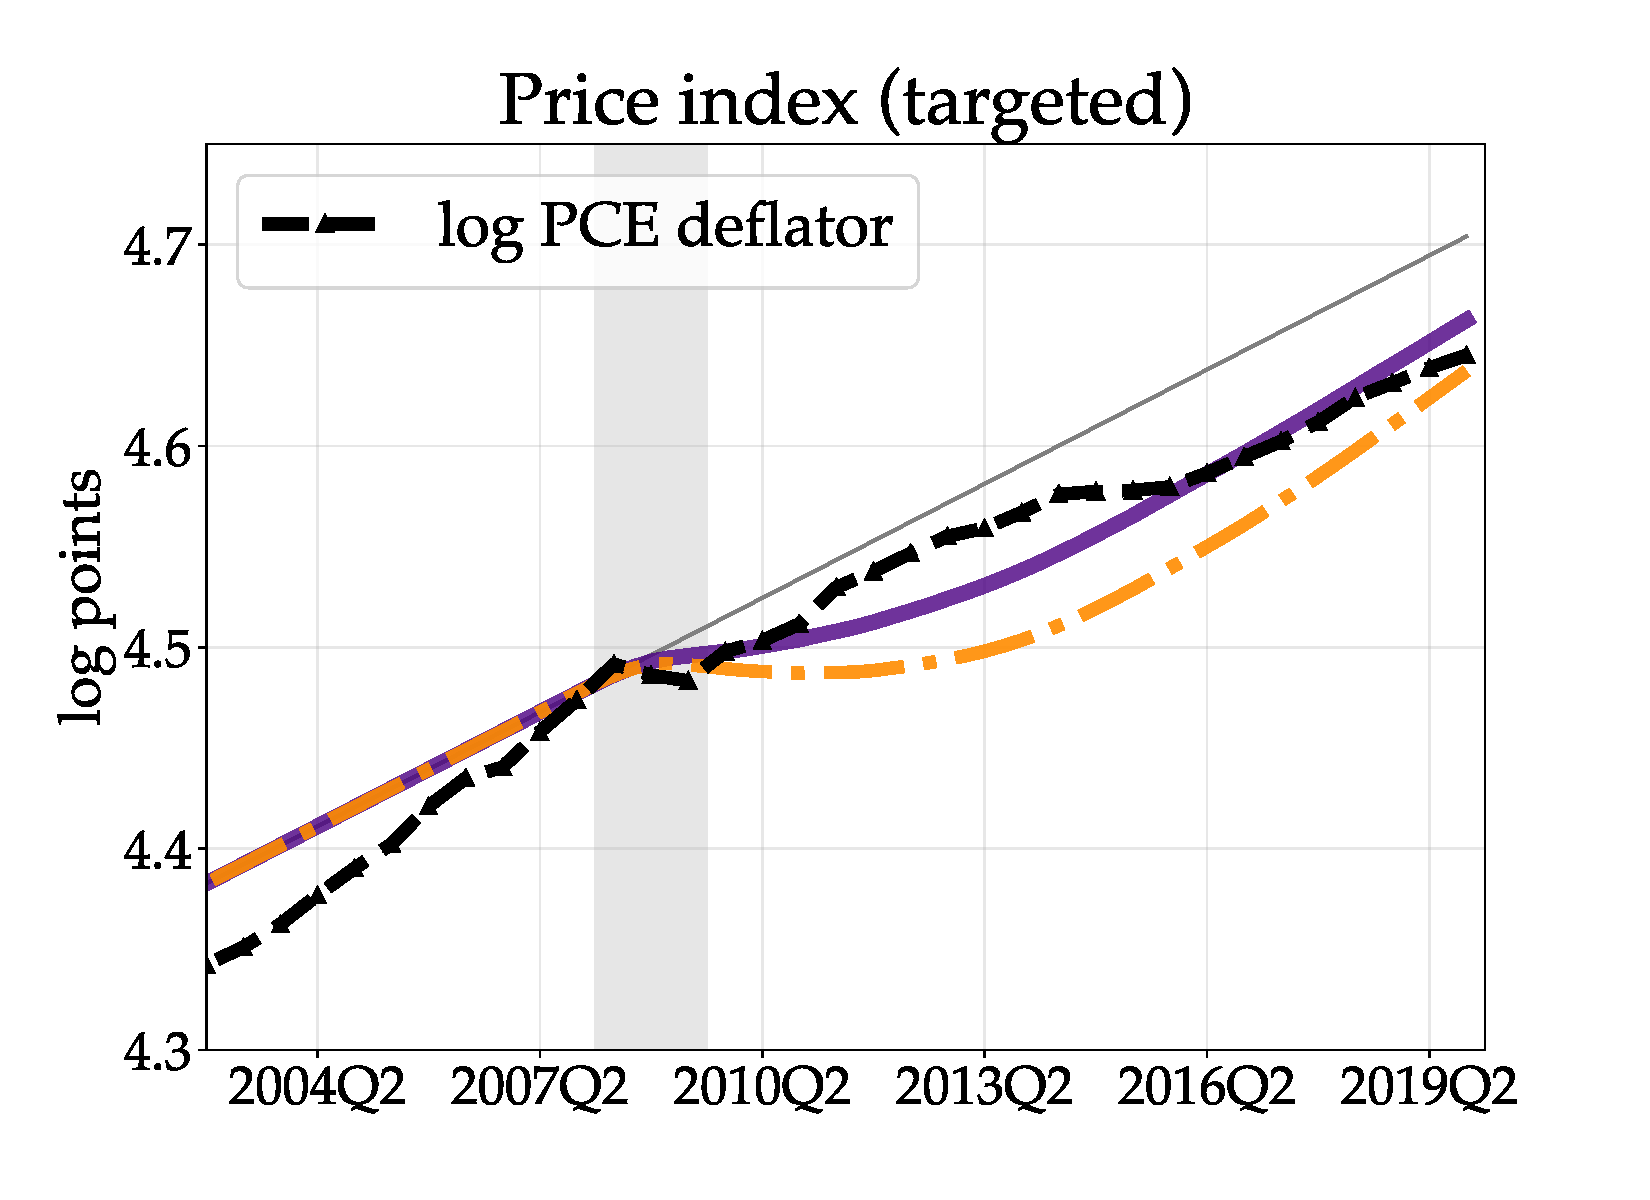
\includegraphics[scale=.29]{text/chapter1/Figures/GR_sim/Cleaner/price_vs_data_large_new}
 \label{fig:b}
\end{minipage}
\medskip
\begin{minipage}{0.51\textwidth}
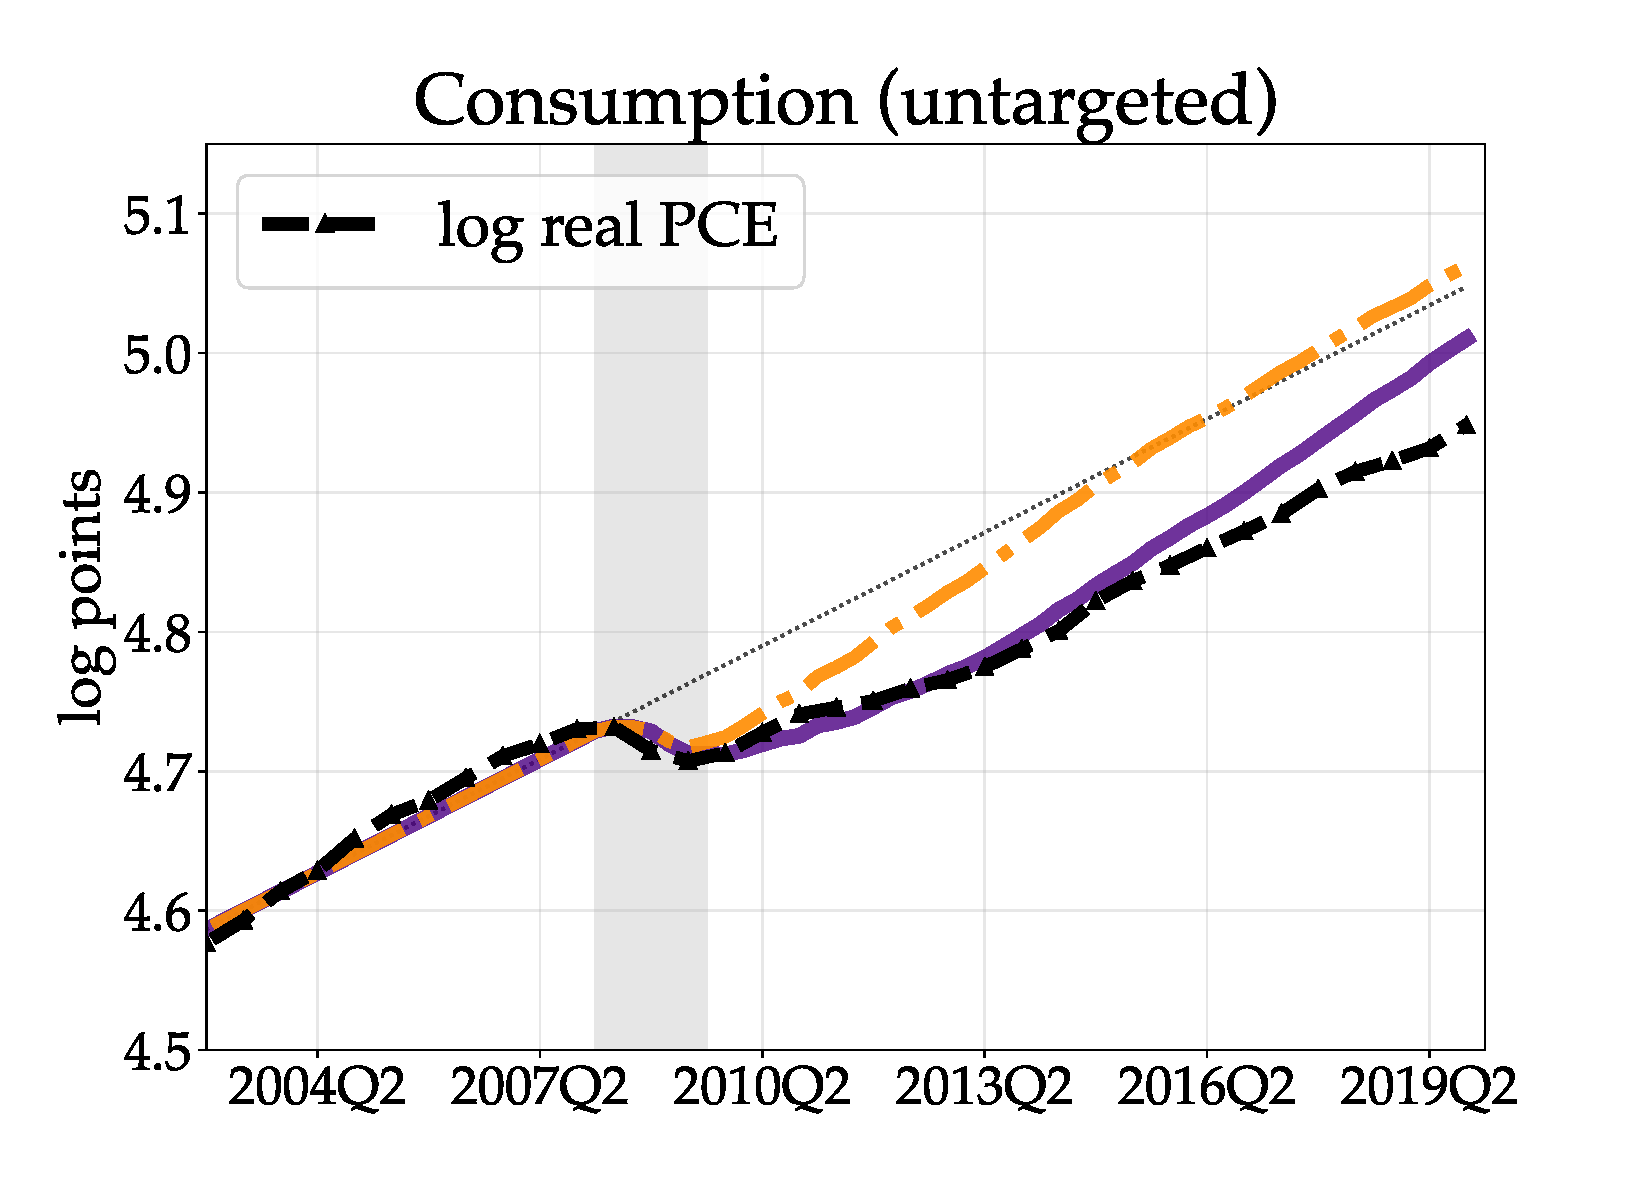
\includegraphics[scale=.29]{text/chapter1/Figures/GR_sim/Cleaner/Consumption_vs_data_large_new}
\label{fig:c}
\end{minipage}\hspace*{\fill}
\begin{minipage}{0.51\textwidth}
\includegraphics[scale=.29]{text/chapter1/Figures/GR_sim/Cleaner/Output_vs_data_large_new}
 \label{fig:d}
\end{minipage}
\medskip
\begin{minipage}{0.51\textwidth}
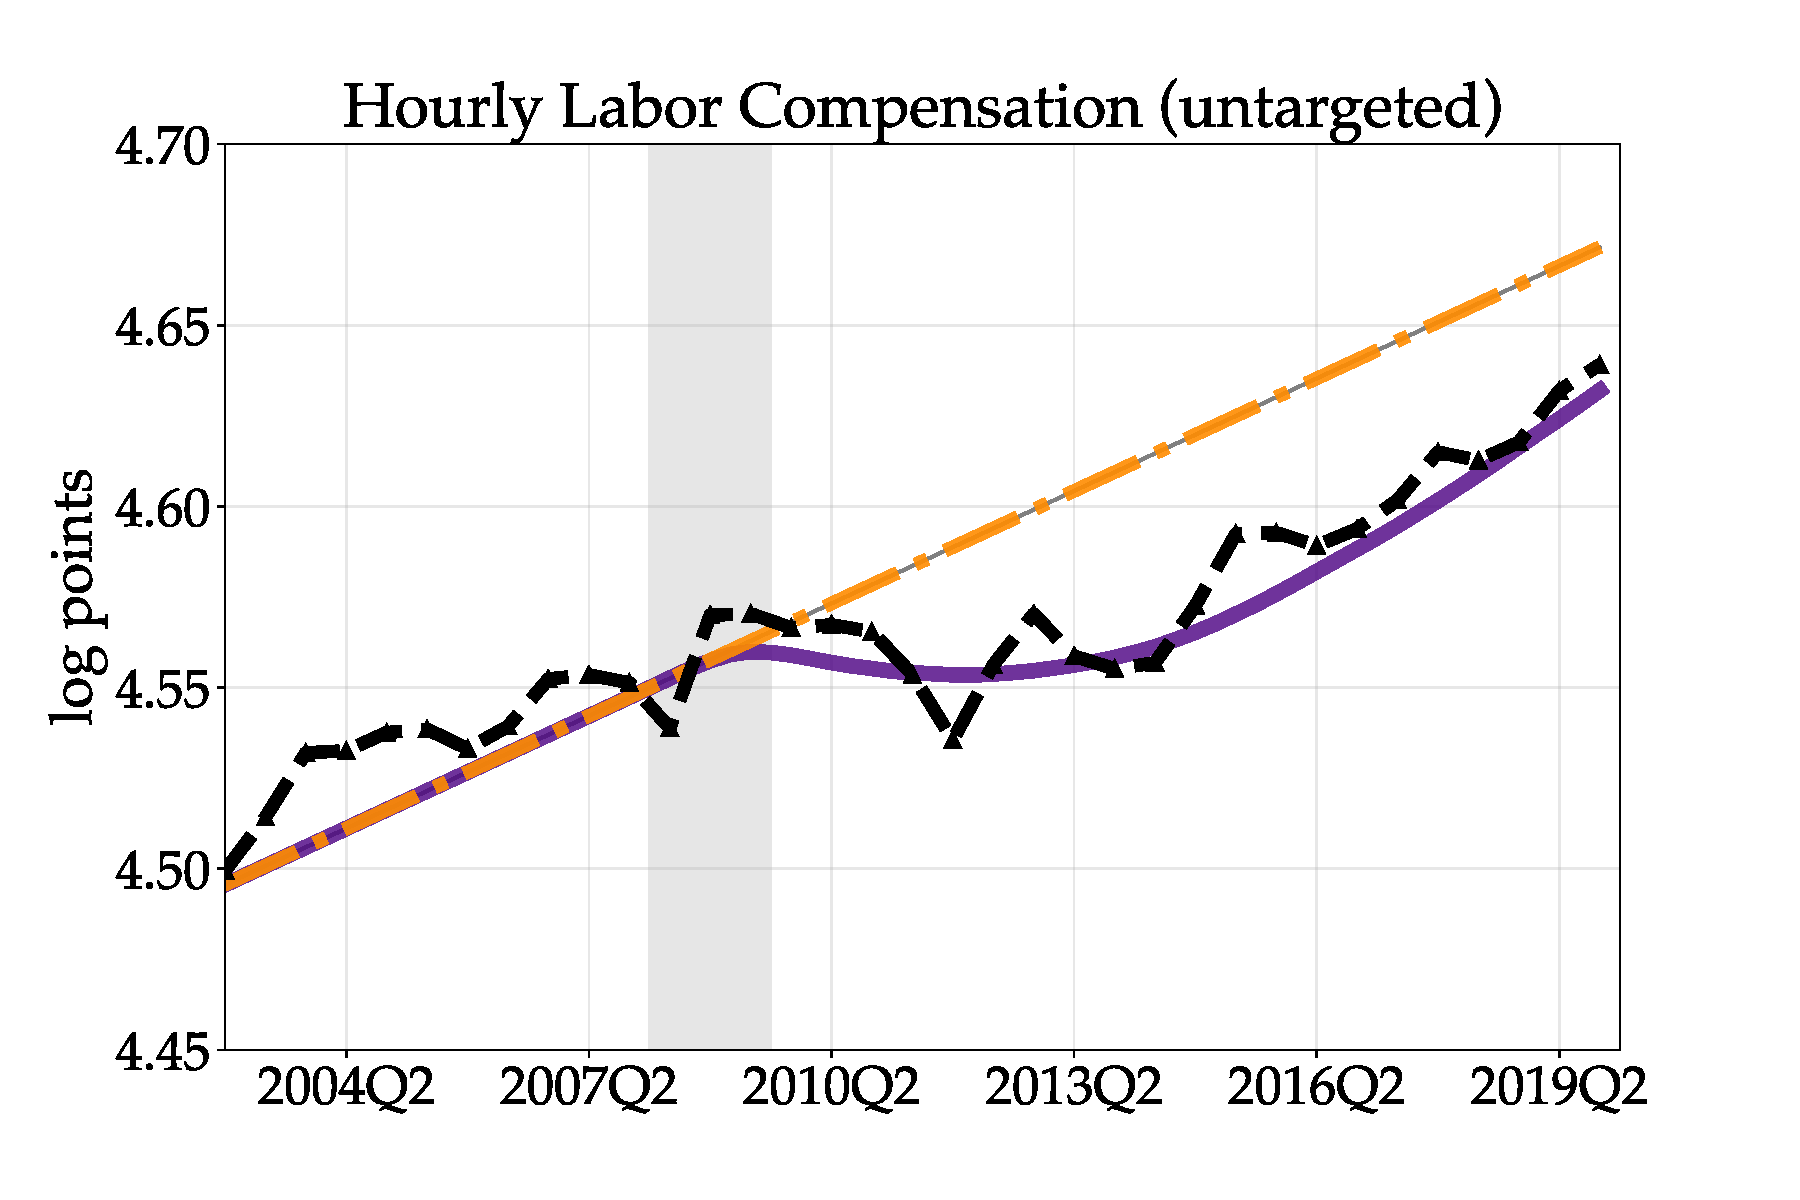
\includegraphics[scale=.29]{text/chapter1/Figures/GR_sim/Cleaner/hourly_comp_vs_data_large_new}
 \label{fig:e}
\end{minipage}\hspace*{\fill}
\begin{minipage}{0.51\textwidth}
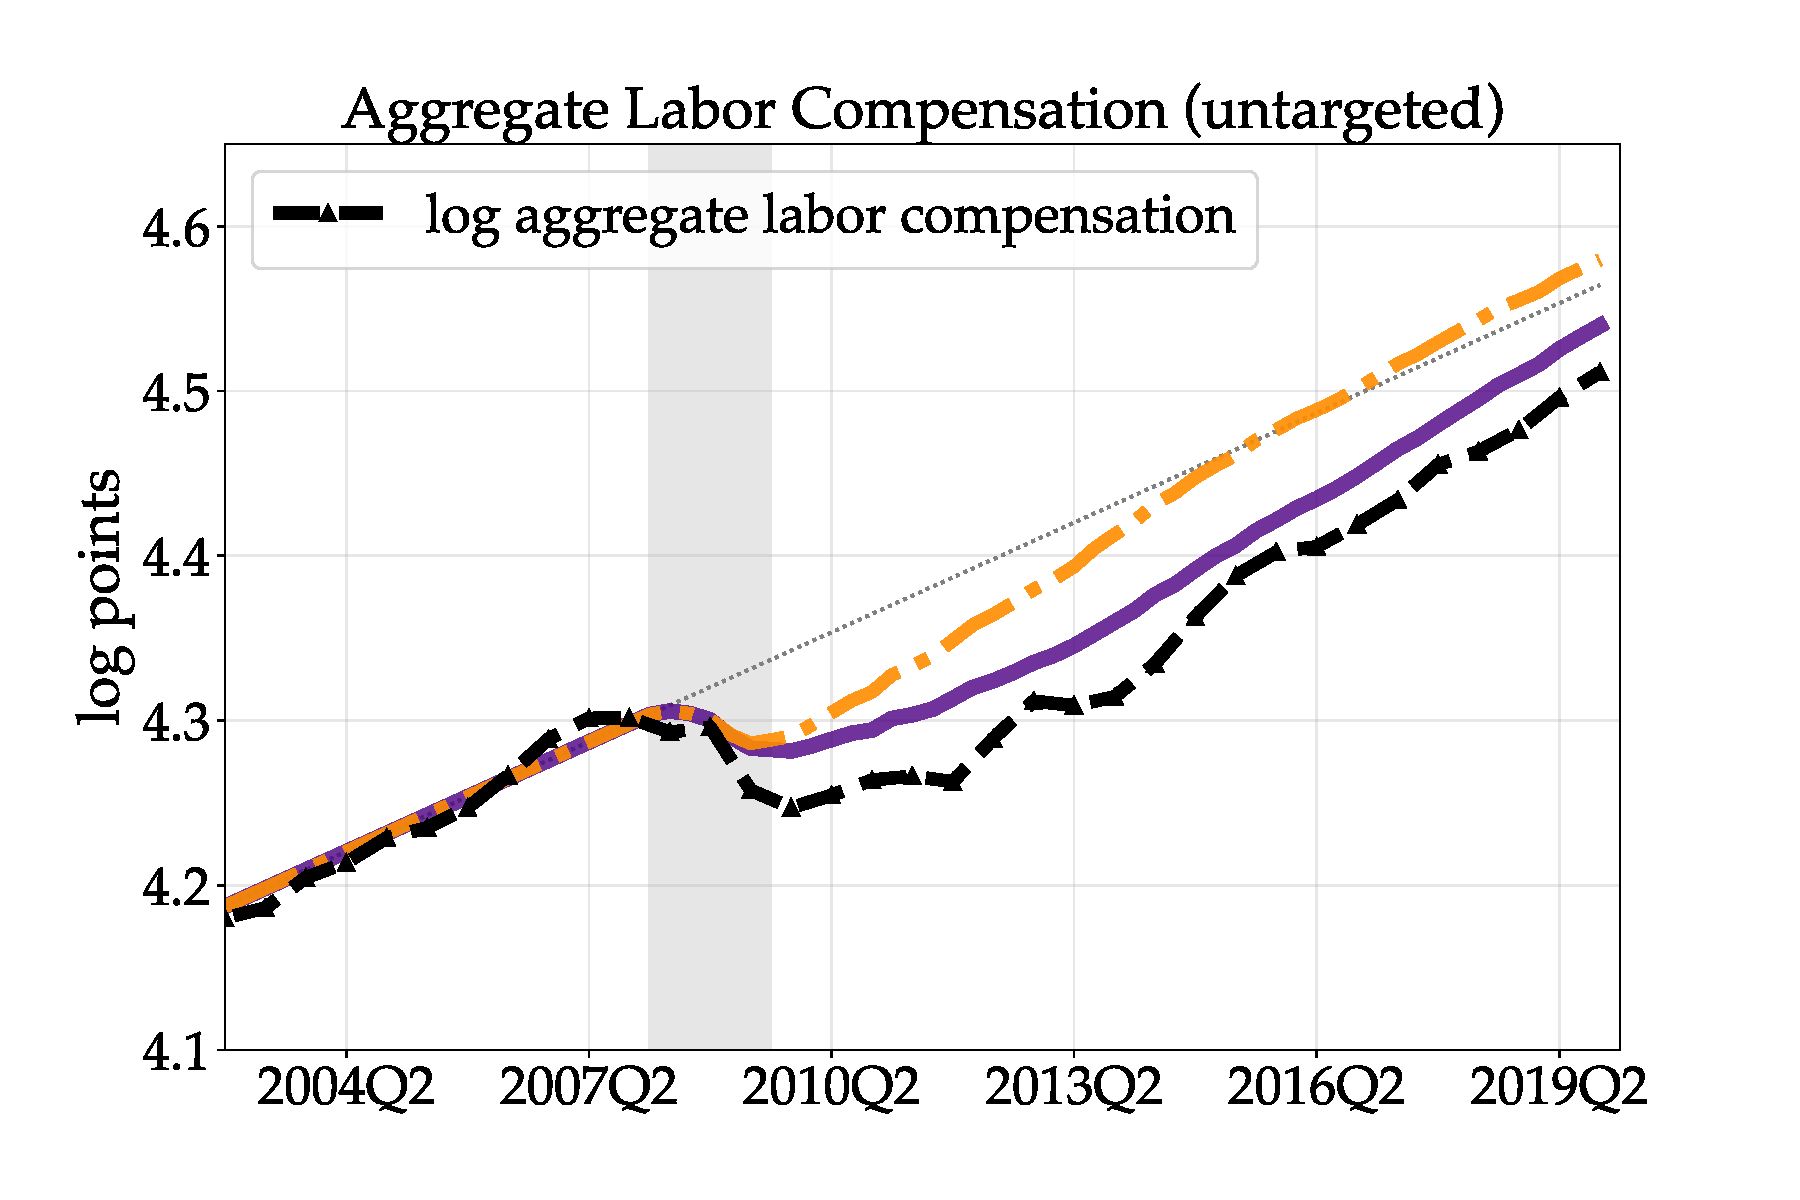
\includegraphics[scale=.29]{text/chapter1/Figures/GR_sim/Cleaner/labor_comp_vs_data_large_new}
 \label{fig:f}
\end{minipage}
\caption{Great Recession: Model vs Data (with trend)}
\floatfoot{Note: This figure plots the responses from figure \ref{NonTarget} with the trend.}
\label{NonTarget_with_trend}
\end{figure}


Figure \ref{Estimatedshks} plots the estimated shocks, the unemployment rate, and the nominal rate against the data under the baseline model and the model without scarring. Figure \ref{NonTarget} plots the key aggregate variables against their detrended observed counterpart in the data and \ref{NonTarget_with_trend} plots the model responses against the data without detrending. Only the unemployment rate and price index are targeted. 

Overall, unemployment scarring explains a substantial share of slow recovery following the Great Recession. In particular, scarring allows the model to match the path of the PCE and GDP until the beginning of 2015. Furthermore, the model under predicts the response of aggregate labor compensation likely due to the absence of labor force participation in the model. The path of hour labor compensation is matched especially well and provides macroeconomic validation that for unemployment scarring. Without unemployment scarring, the response of PCE, GDP, and aggregate labor compensation exhibit a 'V' shaped recovery as it mirrors the response of the unemployment rate. Unemployment scarring generates a persistent decline in labor productivity without a prolonged increase in the unemployment rate. This allows model to produce an income response that is significantly more persistent than the response of unemployment. 





\subsection{Debt to GDP during the Great Recession}


Having shown that the model can replicate the sluggish recovery from The Great Recession, in this section I evaluate the extent to which human capital losses increased debt to GDP during and after the Great Recession. Figure \ref{DebtGDP_sim} plots the simulated path of debt to GDP and tax revenues under the baseline model and the model without scarring. The model suggests that, by 2019, unemployment scarring increased debt to GDP by 5.5 $\%$ points. Human capital losses cause persistent losses in GDP as well as tax revenues which in turn increases debt.

\begin{figure}[!ht]
    \centering
   \begin{minipage}{0.48\textwidth}
        \centering
        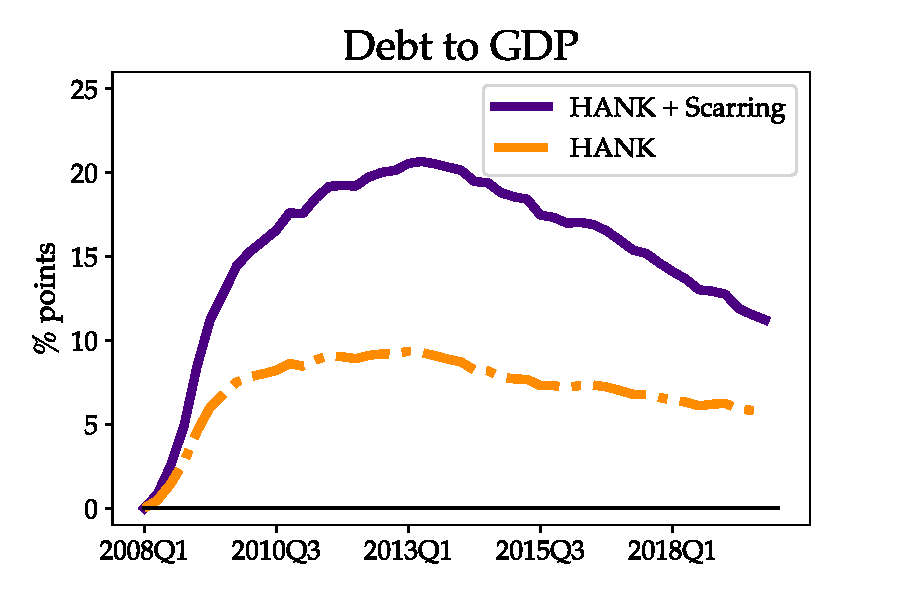
\includegraphics[scale=.57]{text/chapter1/Figures/GR_sim/debt2GDP_GR} % first figure itself
    \end{minipage}\hfill
    \begin{minipage}{0.48\textwidth}
        \centering
        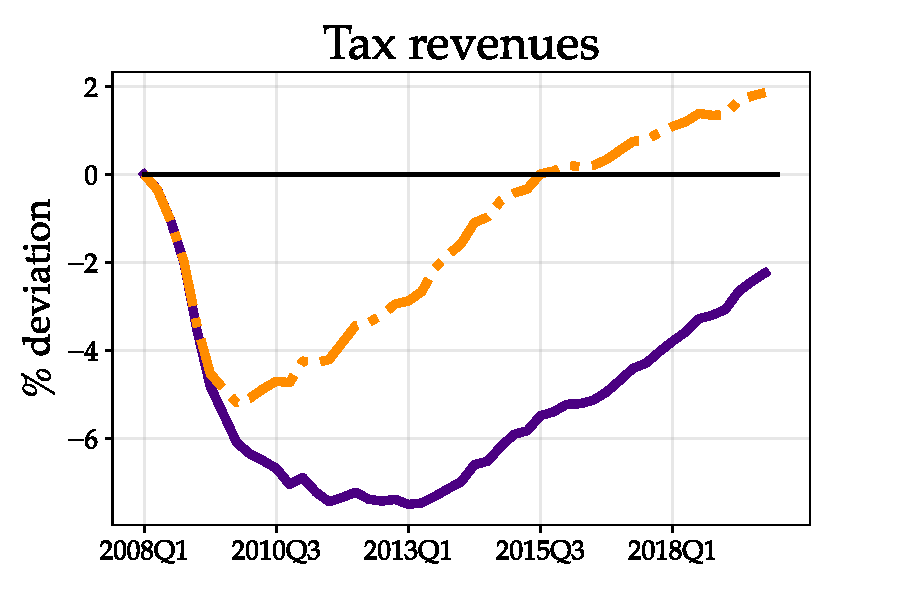
\includegraphics[scale=.57]{text/chapter1/Figures/GR_sim/tax_rev} % second figure itself
    \end{minipage}
    \caption{The response of debt to GDP and tax revenues}
    \label{DebtGDP_sim}
\end{figure}




\subsection{Income Inequality during the Great Recession}

Unemployment scarring increases the dispersion in human capital during a recession. As households become unemployment and later find reemployment at a lower wage, the variance of the distribution of wages increases persistently as the re-accumulation of human capital is slow.  Figure \ref{Gini_GR} shows that unemployment scarring allows the model to generate a near-permanent response in the Gini index of income that is consistent with the data. 


\begin{figure}[!ht!]
\begin{center}
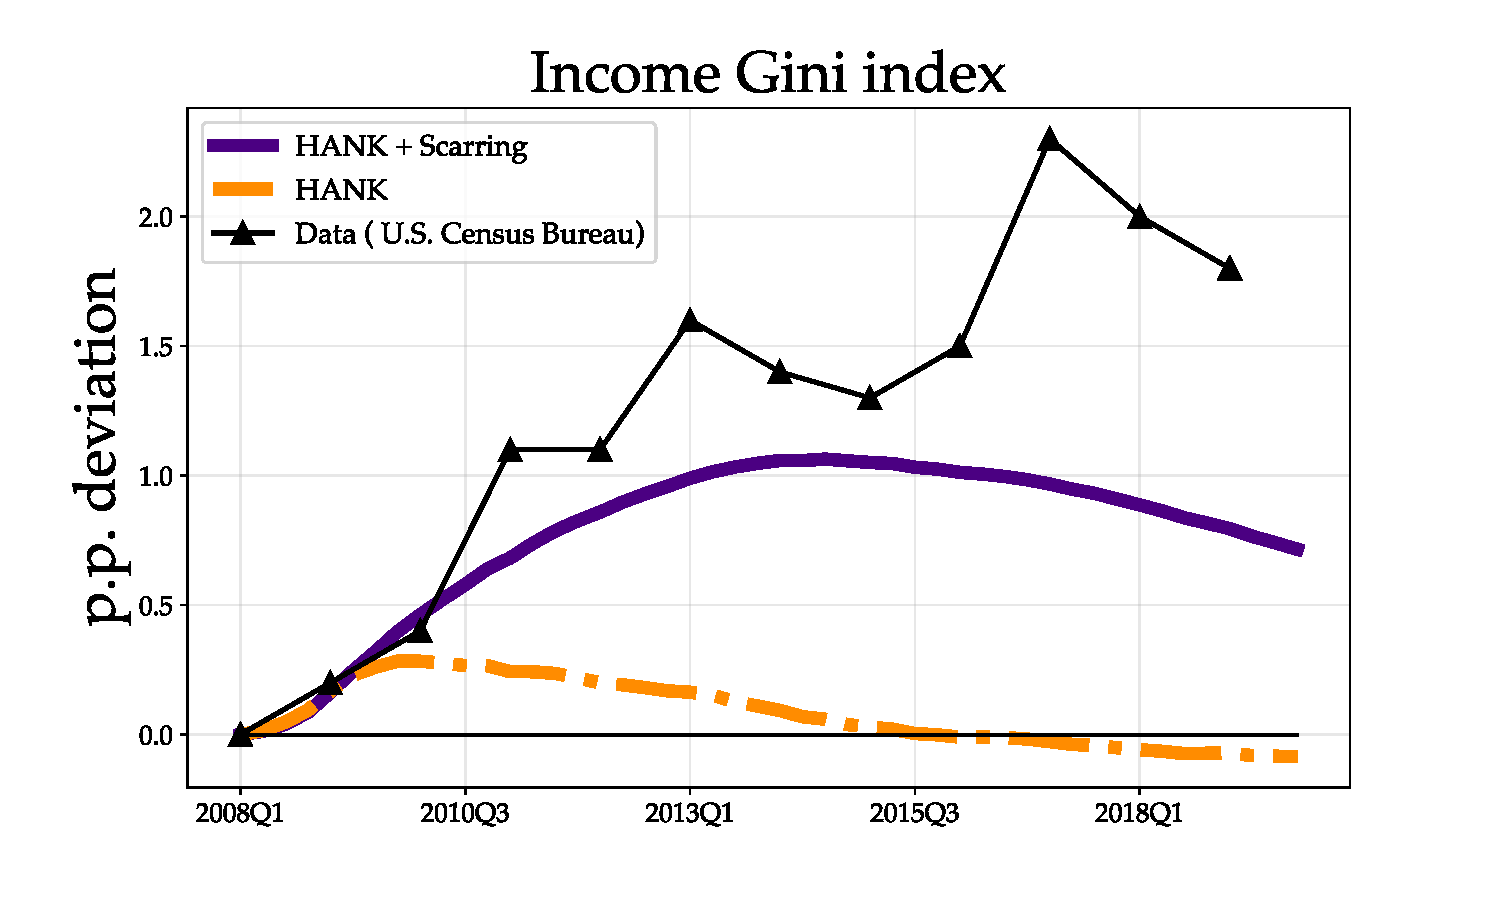
\includegraphics[scale=0.5]{text/chapter1/Figures/GR_sim/income_gini}
\end{center}
\caption{Gini Coefficient: Model vs Data}
 \label{Gini_GR}
\end{figure}

